\documentclass[tc,openright]{iiufrgs}
\usepackage[T1]{fontenc}        % pacote para conj. de caracteres correto
\usepackage[utf8]{inputenc}   % pacote para acentua\c c\~ ao
\usepackage{graphicx}           % pacote para importar figuras
\usepackage{times}              % pacote para usar fonte Adobe Times
\usepackage{multirow}
\usepackage{subfigure}
\usepackage{listings}
\usepackage{scalefnt}
\usepackage[brazilian]{babel}
\usepackage{tabularx}
%\usepackage{hyperref}
%\usepackage{float}

\bibliographystyle{abnt}
%\bibliographystyle{apalike}

\hyphenation{en-si-na-men-tos a-gra-de-ci-men-to de-se-nha-dos}

\title{Framework AOP utilizando técnicas de Byte Code Engineering}

\author{Bento}{Nicolas}

\advisor[Prof.]{Torres}{Márcio}

\date{fevereiro}{2014}

\location{Rio Grande}{RS}

\renewcommand{\nominata}{
        UNIVERSIDADE FEDERAL DO RIO GRANDE\\
        Reitor: Prof. Cleuza Maria Sobral Dias\\
        Pró-Reitor de Graduaçăo: Prof. Denise Varella Martinez\\
        Coordenador do curso: Prof. Tiago Lopes Telecken\\
}

\keyword{AOP, Byte Code Engineering, Meta-programação, Framework, Soc}

\begin{document}

\maketitle

\begin{folhadeaprovacao}
Monografia sob o título \textit{"Framework AOP utilizando técnicas de Byte Code Engineering"}, defendida por Nicolas Dias Bento e aprovada em ?? de ?? de ???, em Rio Grande, estado do Rio Grande do Sul, pela banca examinadora constituída pelos professores:
 \assinatura{Prof. Márcio Torres\\ Orientador}
 \assinatura{Prof. NOME\\ IFRS - Campus Rio Grande }
 \assinatura{Prof. NOME\\ IFRS - Campus Rio Grande } 
\end{folhadeaprovacao}

\clearpage

\begin{flushright}
\mbox{}\vfill
{\sffamily\itshape
"A mente que se abre a uma nova ideia jamais volta ao seu tamanho original."\\}
--- \textsc{Albert Einstein}
\end{flushright}

\chapter*{Agradecimentos}

Agradecimentos ...

\tableofcontents

\begin{listofabbrv}{SPMD}
	\item[AOP] \textit{Aspect Oriented Programming} (Programação Orientada a Aspectos)
	\item[SoC] \textit{Separation of concerns} (Separação de Interesses)
	\item[OOP] \textit{Object Oriented Programming} (Programação Orientada a Objetos)
	\item[PARC] \textit{Palo Alto Research Center} (Centro de Pesquisa Palo Alto) 
	\item[SQL] \textit{Structured Query Language} (Linguagem de Consulta Estruturada)
	\item[YAGNI] \textit{You aren’t gonna need it} (Você não vai precisar dele)
	\item[XP] \textit{Extreme Programming} (Programação Extrema)
	\item[Javassist] \textit{Java Programming Assistant} (Assistente de Programação Java)
	\item[BCEL] \textit{Byte Code Engineering Library}
	\item[API] \textit{Application Programming Interface} (Interface de Programação de Aplicativos)
\end{listofabbrv}

\listoffigures

\listoftables

\begin{abstract}

Resumo ...

\end{abstract}

\chapter{Introdução}
\section{Objetivo}
\section{Motivação}
\section{Resumo dos capítulos}
 
\chapter{Aspect Oriented Programming}
Neste capítulo será abordado de forma geral o paradigma de programação orientada a aspectos. Será falado um pouco da história deste paradigma, passando de forma objetiva pelos principais conceitos e benefícios, trazendo as informações necessárias para a compreensão superficial deste paradigma.
\section{Definição}
AOP é um paradigma de programação que foi construído tomando como base outros paradigmas (OOP e \textit{procedural programming}) , cujo o principal objetivo seria a modularização de interesses transversais, utilizando um dos paradigmas base na implementação dos interesses centrais. A forma como AOP e o paradigma base se integram se dá com a utilização de aspectos que determinam a forma como os diferentes módulos se relacionam entre si na formação do sistema final \cite{laddad2003aspectj}.
\section{História}
Após um grande período de estudos, pesquisadores chegaram a conclusão que para desenvolver um software de qualidade era fundamental separar os interesses do sistema, ou seja, deveria então ser aplicado o princípio de \textit{Separation of Concerns} (SoC)\footnote{Para saber mais sobre SoC consulte o Glossário.}. Em 1972, David Parnas escreveu um artigo, que tinha como  proposta aplicar SoC através de um processo de modularização, onde cada módulo deveria esconder as suas decisões de outros módulos.Passado alguns anos, pesquisadores continuaram a estudar diversas formas de separação de interesses. OOP foi a melhor, se tratando de separação de interesses centrais, mas quando se tratava de interesses transversais, acabava deixando a desejar. Diversas metodologias — \textit{generative programming, meta-programming, reflective programming, compositional filtering, adaptive programming, subject-oriented programming, aspect oriented programming,} e  \textit{intentional programming} — surgiram como possíveis abordagens para modularização de interesses transversais. AOP acabou se tornando a mais popular entre elas \cite{laddad2003aspectj}.

Em 1997 Gregor Kiczales e sua equipe descreveram de forma sólida o conceito de Programação Orientada a Aspectos, durante um trabalho de pesquisa realizado pelo PARC, uma subsidiária da \textit{Xerox Corporation}. O documento descreve uma solução complementar a OOP, ou seja, seriam utilizados "aspectos" para encapsular as preocupações transversais, de forma a garantir a reutilização por outros módulos de um sistema.Sugeriu também diversas implementações de AOP, servindo como base para a criação do AspectJ\footnote{No final dos anos 90, a Xerox Corporation, transferiu o projeto AspectJ para a comunidade Open Source em eclipse.org.}, uma linguagem AOP muito difundida nos dias de hoje \cite{groves2013aop}.

\begin{figure}[ht]
	\centering
	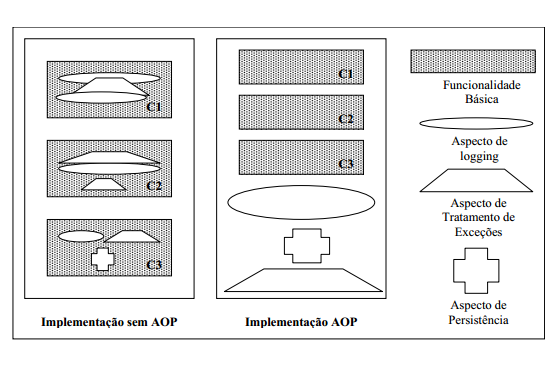
\includegraphics[scale=0.6]{figuras/funcionamentoAOP.png}
	\caption{Funcionamento de AOP.}
	\small{Fonte: Autoria própria.}
	\label{fig:funcionamentoAOP}
\end{figure}

\section{Principais conceitos}

Para entender melhor o funcionamento de AOP, é preciso compreender seus principais conceitos. 

Os 5 principais conceitos de AOP são:

\begin{description}
\item [Aspecto] (\textit{aspect}) - pode ser definido como um interesse transversal, ou seja, interesse onde sua implementação é espalhada por diversos módulos ou componentes de um sistema.
\item [Ponto de junção] (\textit{joinpoint}) - pode ser definido basicamente como pontos bem definidos na execução de um programa.
\item [Ponto de corte] (\textit{pointcut}) - em AOP um \textit{pointcut} pode ser representado como um agrupamento de pontos de junção.
\item [Conselho] (\textit{advice}) - é a implementação de determinado interesse transversal, sendo executado quando determinado \textit{pointcut} é ativado, podendo ser executado antes (\textit{before}), em torno (\textit{around}) ou depois (\textit{after}) da execução de um ponto de junção.
\item [Introdução] (\textit{introduction}) - é quando um aspecto introduz algumas mudanças em classes, interfaces , métodos. Por exemplo, pode-se acrescentar uma variável ou método a uma classe existente  \cite{laddad2003aspectj}.
\item [Combinador] (\textit{weaver}) - é a ferramenta responsável pela combinação dos interesses centrais com os interesses transversais do sistema, ou seja,  é o momento de integração destes interesses mediante uma técnica específica.

\end{description}


Pode-se comparar também os conceitos de AOP com os principais conceitos de OOP:

\begin{table}[ht]
	\centering
	\caption{Comparação entre conceitos de AOP e OOP \cite{jacobson2004aspect}.}
	
	\begin{tabular}[h]{c c l}
		\hline 
		\textbf{AOP} & \textbf{OOP} \\
		\hline
		\textit{Aspect}&Classe \\
		\textit{Advice}&Método \\
		\textit{Joinpoint}&Atributo \\
		\hline
	\end{tabular}
	\label{tab:comparacaoAOPOOP}
\end{table}

\textit{Pointcut} não se encaixa em nenhum conceito de orientação a objetos, mas podemos comparar um \textit{pointcut} com um gatilho (\textit{trigger}) da linguagem SQL (\textit{Structured Query Language}) \cite{jacobson2004aspect}.

\section{Benefícios}

De forma geral pode-se dizer que todo paradigma possui seus prós e contras, sendo assim difícilmente será encontrada uma metodologia que resolva todos os problemas da melhor maneira. Com AOP não é diferente, mas deve-se considerar sua larga escala de benefícios:

\begin{itemize}
\item Separação de interesses e Alta modularização - com AOP pode-se separar o projeto em módulos responsáveis por implementar apenas os interesses centrais do sistema, possuindo assim um acoplamento mínimo que extingui o codigo duplicado, fazendo com que o sistema fique muito mais fácil de entender e manter, colocando os interesses transversais (aspectos) em módulos completamente diferentes \cite{laddad2003aspectj}.
\item Fácil evolução - utilizando AOP o sistema fica muito mais flexível quando se trata da adição de novas funcionalidades, fazendo com que a resposta às exigências se tornem mais rápidas.
\item Foco na prioridade - o arquiteto do projeto pode se concentar nos requisitos básicos atuais do sistema, os novos requisitos que abordam interesses transverssais podem ser tratados fácilmente com a criação de novos aspectos. AOP trabalha em harmonia com metodos agéis, por exemplo apóia a prática YAGNI (\textit{"You aren’t gonna need it"}) \footnote{Em português significa "Você não vai precisar dele". Para saber mais sobre YAGNI consulte o Glossário.}, do \textit{Extreme Programming} (XP)\footnote{É um dos métodos agéis mais utilizados na atualidade.} \cite{laddad2003aspectj}.
\item Maior reutilização de código - a chave para a reutização de código definitiva é uma implementação flexível, com AOP é possível pois cada aspecto é implementado como um módulo distinto, se tornando adaptavél a implementações equivalentes convencionais \cite{laddad2003aspectj}. 
\item Aumento na produtividade - o ciclo do projeto se torna mais rápido, a grande reutilização usada em AOP, faz com que o tempo de desenvolvimento seja reduzido, diminuindo também o tempo de implantação e o tempo de resposta às novas exigências de mercado \cite{laddad2003aspectj}. 
\item Redução de custos e aumento da qualidade - com a implementação dos interesses transversais em módulos distintos, o custo de implementação cai bastante, fazendo com que o desenvolvedor concentre-se mais nos interesses centrais, criando um produto de qualidade e com o custo reduzido.
\end{itemize}

\section{Considerações finais}

\chapter{Bytecode Engineering}
Neste capítulo serão abordados alguns conceitos fundamentais de bytecode, também será definida a técnica de Bytecode Engineering, apresentando algumas vantagens em sua utilização e ferramentas que podem ser utilizadas para aplicar esta técnica. 

\section{Fundamentos de bytecode}

Basicamente pode-se dizer que bytecode é a linguagem intermediária entre o código fonte e o código de máquina, que faz com que os programas Java possam ser executados em múltiplas plataformas. O documento responsável pela definição de bytecode é a Especificação da Máquina Virtual Java (\textit{Java Virtual Machine Specification})\footnote{Pode ser acessada em : http://docs.oracle.com/javase/specs/jls/se8/jls8.pdf} que descreve também os conceitos da linguagem, formato dos arquivos de classes, os requisitos da \textit{Java Virtual Machine} (JVM), entre outros \cite{kalinovsky2004covert}.

A JVM que executa sobre o sistema operacional, é responsável pelo ambiente de execução dos programas Java, sendo também a responsável pela conversão de instruções de bytecode Java em instruções nativas de máquina \cite{stark2001java}.

\section{Definição}
Bytecode Engineering é uma técnica normalmente utilizada para criação, manipulação e modificação de classes Java compiladas à nível de bytecode. Muitas tecnologias  utilizam esta técnica para otimizar, ou melhorar classes já existentes.
\section {Vantagens}

Dentre as principais vantagens em utilizar bytecode engineering estão:

\begin{itemize}
\item Consegue-se manipular o bytecode sem a necessidade de recompilação, ou obtenção do código fonte original.
\item O bytecode pode ser gerado ou instrumentado por \textit{class loader} em tempo real, enquanto as classes são carregadas em uma JVM \cite{kalinovsky2004covert}.
\item É muito mais fácil e rápido automatizar a geração de bytecode por ser um processo mais baixo nível e também por não haver a necessidade de execução do compilador, ao contrário da geração de código fonte que possui alguns passos a mais no seu processo, e também necessita da execução do compilador \cite{kalinovsky2004covert}.
\item Instrumentar métodos, tendo como objetivo a inserção de lógica adicional, que não necessita estar nos arquvos de código fonte. Por exemplo, pode-se deixar no arquivo fonte apenas os interesses centrais do sistema, e incluir os interesses transversais utilizando bytecode engineering. 
\end{itemize}

\section{Ferramentas}

Pode-se dizer que a manipulação de bytecode é uma tarefa complexa, pois bytecode é uma linguagem de baixo nível, e o aprendizado desta linguagem para programadores de alto nível, tende a ser muito lenta, fazendo com que seja inviável o seu aprendizado dentro do escopo de um projeto.

Pensando neste problema, foram criadas algumas bibliotecas que tornam o processo de manipulação de bytecode mais alto nível, facilitando o seu aprendizado. As bibliotecas mais utilizadas que aplicam a técnica de \textit{bytecode engineering} são: \textit{Javassist}, \textit{Byte Code Engineering Library (BCEL)} e \textit{ASM}.

\subsection {Javassist}

Javassist (Assistente de Programação Java) é uma biblioteca de classes utilizada na manipulação de bytecodes em Java, permitindo que classes sejam criadas em tempo de execução e manipuladas no tempo de carregamento da JVM. A principal diferença do Javassist para outros manipuladores de bytecode, é que javassist possui  API (\textit{Application Programming Interface}) no nível de código fonte e no nível de bytecode \cite{javassist}.
\subsection {BCEL}
 BCEL tem como objetivo oferecer aos usuários (desenvolvedores) uma maneira conveniente de analizar, criar, manipular arquivos de classe Java (binário). No BCEL as classes são representadas por objetos que contêm todas as suas informações (métodos, campos e instruções de bytecode) \cite{bcel}.
\subsection {ASM}
ASM é uma estrutura de manipulação de bytecode Java. Ela pode ser usada para gerar classes dinamicamente, diretamente na forma binária, ou modificar dinamicamente as classes em tempo de carregamento, ou seja, antes de serem carregados pela JVM. ASM oferece funcionalidades semelhantes ao BCEL, mas é muito menor e mais rápido do que essa ferramenta \cite{asmjavasource}.

\section{Considerações finais}

\chapter{Metaprogramação}
Neste capitulo serão introduzidos  os princípais conceitos de metaprogramação, falando também dos principais benefícios em aplicar esta metodologia em seus programas. Também é apresentado neste capítulo informações relevantes sobre o uso de anotações e reflexão na linguagem Java.

\section{Definição}

Metaprogramação por sua vez, pode ser definida como sendo um programa de computador que escreve e/ou manipula programas em tempo de execução ou compilação, fazendo com que o programa se adapte a diferentes circunstâncias, podendo controlar, monitorar ou invocar a si mesmo, visando alcançar as funcionalidades desejadas \cite{hazzard2013metaprogramming}.
\section{Benefícios}
O uso de metaprogramação no desenvolvimento de software pode trazer uma série de benefícios tanto para a empresa, quanto para o desenvolvedor, entre alguns dos princípais benefícios estão:

\begin{itemize}
\item Simplicidade - com metaprogramação tem-se a possibilidade de adaptar um único bloco de código a diversas situações, sem a necessidade de geração de código, fazendo com as classes se tornem simples e ao mesmo tempo pequenas em comparação a outros programas que não usam esta abordagem.
\item Adaptação em tempo real - pode-se fazer uma análise minuciosa do programa em tempo de execução, fazendo com que alterações no modelo de dados da aplicação sejam percebidas em tempo real, ou seja, pode-se tornar o sistema altamente configurável sem a necessidade de compilação do projeto.
\end{itemize}

\section{Principais conceitos}
Para entender melhor a metaprogramação, é necessário compreender seus princípios (conceitos) básicos:

\begin{description}
\item [Metalinguagem]  linguagem usada para escrever um metaprograma.
\item [Metaprograma ] representa um conjunto de componentes semelhantes que contém funcionalidades diferentes, que podem ser instanciados através de parametrização de modo a criar uma instância do componente específico \cite{damavsevivcius2008taxonomy}.
\item [Metadados] são dados estruturados ou codificados que descrevem as características das entidades , portando informações que visam auxiliar na identificação,  descoberta, avaliação e gestão das entidades descritas \cite{american1999task}.
\item [Reflexão] é a capacidade de um programa em observar e modificar, possivelmente, a sua estrutura e comportamento, fazendo com que a própria linguagem de programação faça o papel de metalinguagem \cite{malenfant1996tutorial}.
\end{description}

\section{Anotações em Java}
Metadados estão disponíveis na linguagem Java apartir da versão 5,  representados através de anotações (\textit{annotations}), sendo apresentada como uma das principais novidades no lançamento desta versão.
\subsection{Definição}

Uma anotação associa uma informação arbitrária ou um metadado com um elemento de um programa Java. Cada anotação tem um nome e zero ou mais membros. Cada membro tem um nome e um valor, e são
estes pares \textit{nome = valor} que carregam as informações da anotação \cite{flanagan2005java}.

Anotações são um tipo especial de interface, designado pelo caractere \textit{@} que é precedido da palavra-chave \textit{interface}.Anotações são aplicados aos elementos do programa, ou também em outras anotações, com o intuito de fornecer informações adicionais \cite{arnold2000java}.

\subsection{Conceitos}

As anotações em Java possuem alguns conceitos importantes que devem ser compreendidos: 

\begin{description}
\item [Tipo de anotação] (\textit{annotation type}) - O nome de uma anotação, bem como os nomes, tipos e valores padrão de seus membros são definidos pelo tipo de anotação. Um tipo de anotação é essencialmente uma interface Java com algumas restrições sobre seus membros \cite{flanagan2005java}.
\item [Membro de anotação] (\textit{annotation member}) - Os membros de uma anotação são declarados em um tipo de anotação como métodos sem argumentos. O nome do método e o tipo de retorno define o nome e o
tipo do membro \cite{flanagan2005java}.
\item [Anotação marcadora] (\textit{marker annotation}) -É um tipo de anotação que não define membros, ou seja, uma anotação desse tipo traz informações simplesmente pela sua presença ou ausência \cite{flanagan2005java}.
\item [Meta-anotação] (\textit{meta-annotation}) - são anotações utilizadas para descrever o comportamento de um tipo de anotação \cite{horstmann2004core}.
\item [Alvo] (\textit{target}) - elemento do programa que será anotado.
\item [Retenção] (\textit{retention}) - é a especificação do tempo em que a informação contida na anotação é mantida. A especificação deste tempo é feita através de uma meta-anotação \cite{flanagan2005java}.
\end{description}

\subsection{Utilidades}

Utilizando anotações em java pode-se adicionar diversas funcionalidades e recursos ao software, sem que haja depêndencias com as classes.

 Dentre as principais utilidades em usar anotações estão:

\begin{itemize}
\item Fornecer informações ao compilador - por exemplo, pode-se utilizar este recurso para detectar erros especifícos em determinada parte do programa em tempo de compilação, também pode-se informar ao compilador que ignore determinados tipos de avisos, etc.
\item Processamento em tempo de compilação - normalmente utiliza-se este recurso através de ferramentas capazes de processar anotações, com o intuito de gerar código, arquivos, etc. 
\item Processamento em tempo de execução - pode-se utilizar para marcar elementos, com o objetivo de ler sua estrutura (tipo, modificadores de acesso,etc) através de reflexão em tempo de execução, fazendo com que o programa se adapte com determinadas situações.
\end{itemize}
\subsection{Exemplo}

Na figura \ref{fig:criandoAnotacao} é mostrado como criar uma anotação básica, que terá como alvo uma classe, e estará visível em tempo de execução, e também irá possuir um membro cujo tipo é uma \textit{String}.

\begin{figure}[ht]
	\centering
	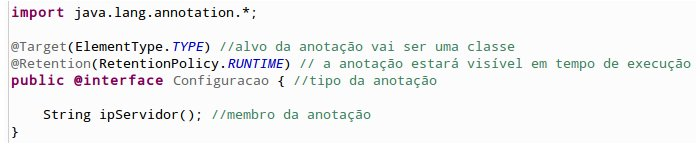
\includegraphics[scale=0.6]{figuras/criandoAnnotation.jpg}
	\caption{Criando uma anotação.}
	\small{Fonte: Autoria própria.}
	\label{fig:criandoAnotacao}
\end{figure}

Na figura \ref{fig:usandoAnotacao} é mostrado como utilizar a anotação criada na figura \ref{fig:criandoAnotacao}.

\begin{figure}[ht]
	\centering
	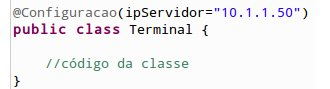
\includegraphics[scale=0.6]{figuras/usandoAnnotation.jpg}
	\caption{Utilizando uma anotação.}
	\small{Fonte: Autoria própria.}
	\label{fig:usandoAnotacao}
\end{figure}

Para ler as informações de uma anotação visível em tempo de execução é necessário consultar a API de reflexão do \textit{java.lang.reflect}.

\section{Reflexão em Java}
Na linguagem Java pode-se utilizar reflexão por meio do pacote \textit{java.lang.reflect}, juntamente com o pacote \textit{java.lang} que contém as classes \textit{Class} e \textit{Package}, e \textit{java.lang.annotation} que faz referência à classe \textit{Annotation}. Este conjunto de pacotes oferecem uma variedade de classes responsáveis pela leitura e modificação da estrutura de um programa em tempo de execução.

\subsection{Aplicações}

Normalmente utiliza-se reflexão para tomar alguma decisão com base na estrutura do programa, ou apenas mostrar informações sobre ela, ou seja,  utiliza-se o(s) pacote(s) de reflexão do Java para descobrir diversos tipos de informações relacionadas com a estrutura de classes, métodos, atributos e etc. Também pode-se utilizar reflexão para instânciar objetos de um tipo determinado, invocar método(s) de uma classe específica, ler anotações, entre outros.

\subsection{Funcionamento}

A reflexão em um programa Java tem inicio apartir de um objeto do tipo \textit{Class}. Com um objeto do tipo \textit{Class} pode-se ober sua lista completa de membros(métodos, atributos) e informações sobre eles, podendo descobrir também todos os tipos desta classe(interfaces que implementa, classes que estende), e descobrir informações sobre a própria classe, como os modificadores aplicados a ela (\textit{public}, \textit{protected}, \textit{private}, etc) \cite{arnold2000java}.

\subsection{Lendo anotações}

Os pacotes utilizados para reflexão possuem uma API \footnote{Visite: "http://docs.oracle.com/javase/7/docs/api/"  para saber mais sobre a api.} de fácil entendimento, e que oferecem suporte à leitura de anotações.

\begin{figure}[ht]
	\centering
	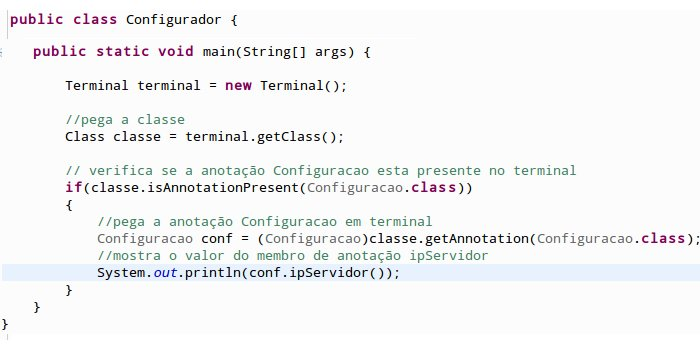
\includegraphics[scale=0.6]{figuras/lendoAnnotation.jpg}
	\caption{Lendo informações de uma anotação.}
	\small{Fonte: Autoria própria.}
	\label{fig:lendoAnotacao}
\end{figure}

Na figura \ref{fig:lendoAnotacao} é mostrado como ler anotações presentes em classes, e também como ler informações presentes nos membros de uma anotação.

\section{Considerações finais}

\chapter{Ferramentas utilizadas}

\chapter{Soluções Existentes}

\section{PostSharp}

\section{AspectJ}

\chapter{O Framework}

\section{Análise e projeto}

\section{Implementação}

\chapter{Estudo de caso - Instrumentação}

\chapter{Conclusão}

Conclusões ...

\bibliography{bibliografia}

\chapter*{Glossário}

\begin{description}
	\item[SoC] è um princípio de projeto, criado com a finalidade de subdividir o problema em conjuntos de interesses tornando a resolução do problema mais fácil.Cada interesse fornece uma funcionalidade distinta, podendo ser validado independentemente das regras negócio \cite{pressman2010engineering}.
	\item [YAGNI] é um princípio de projeto, bastante usado em equipes XP , cuja principal finalidade é implementar apenas o necessário.
	\item[Extreme Programming] XP é um estilo de desenvolvimento de software com foco em excelentes técnicas de programação, comunicação clara e trabalho em equipe, que permite grande produtividade no desenvolvimento \cite{beck2004extreme}.
\item [Decorator] é um padrão de projeto estrutural, cujo principal objetivo é adicionar funcionalidades a um objeto dinamicamente.
\item [Proxy] é um padrão de projeto estrutural, cujo principal objetivo é controlar as chamadas a um objeto através de outro objeto de mesma interface.
\end{description}

\appendix

\end{document}

